% !TeX spellcheck = cs_CZ
\begin{example}
  Generujte signál s lineárně rostoucím kmitočtem "\texttt{chirp signál}", maximální kmitočet
  $f_{max} = 20 Hz$, amplituda $A = 1$, vzorkovaný kmitočtem $f_s = 64 Hz$.

    {\centering
     \begin{tabular}{c}
         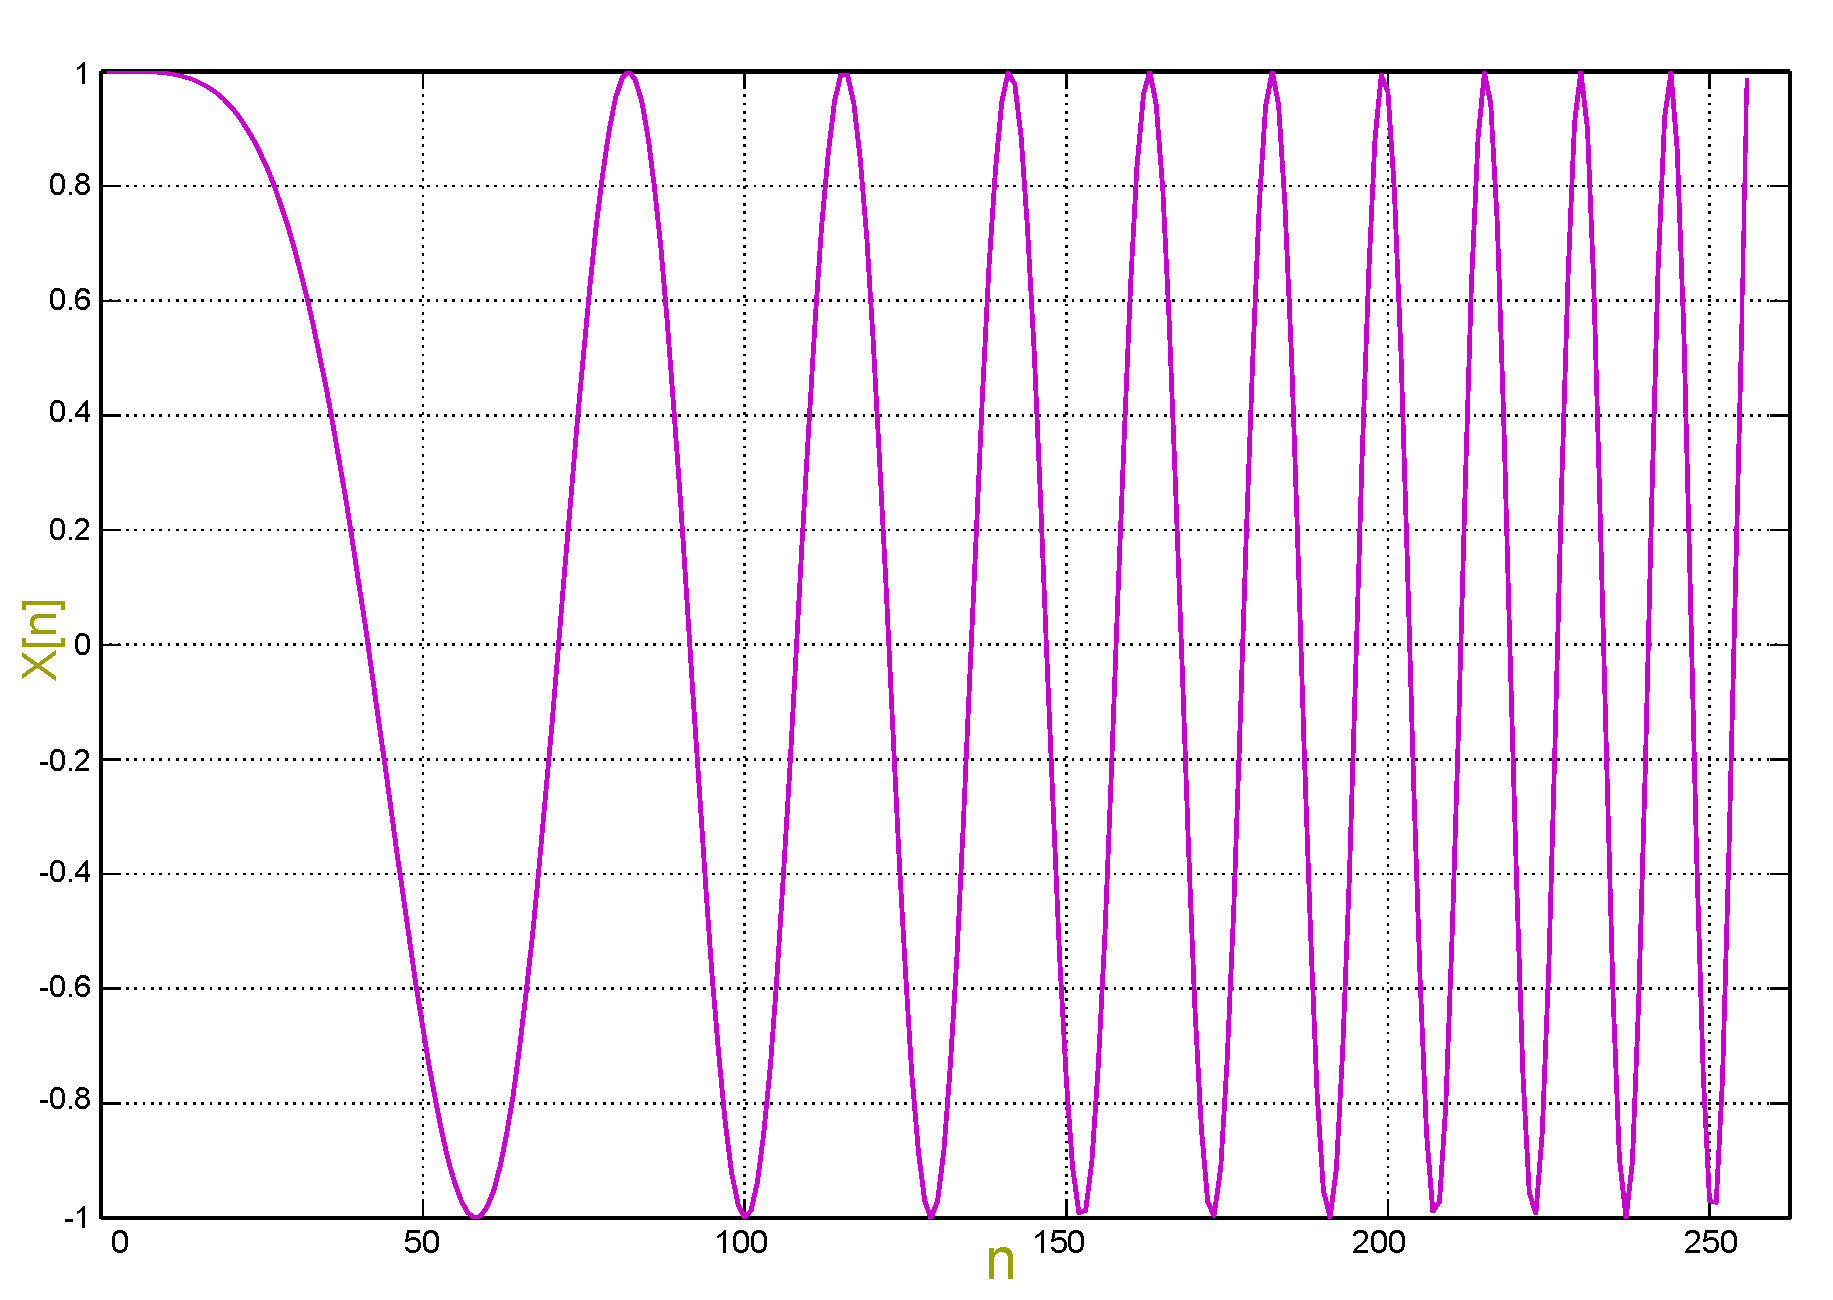
\includegraphics[width=0.8\linewidth]{Chirp_signal_plot.pdf}  \\
         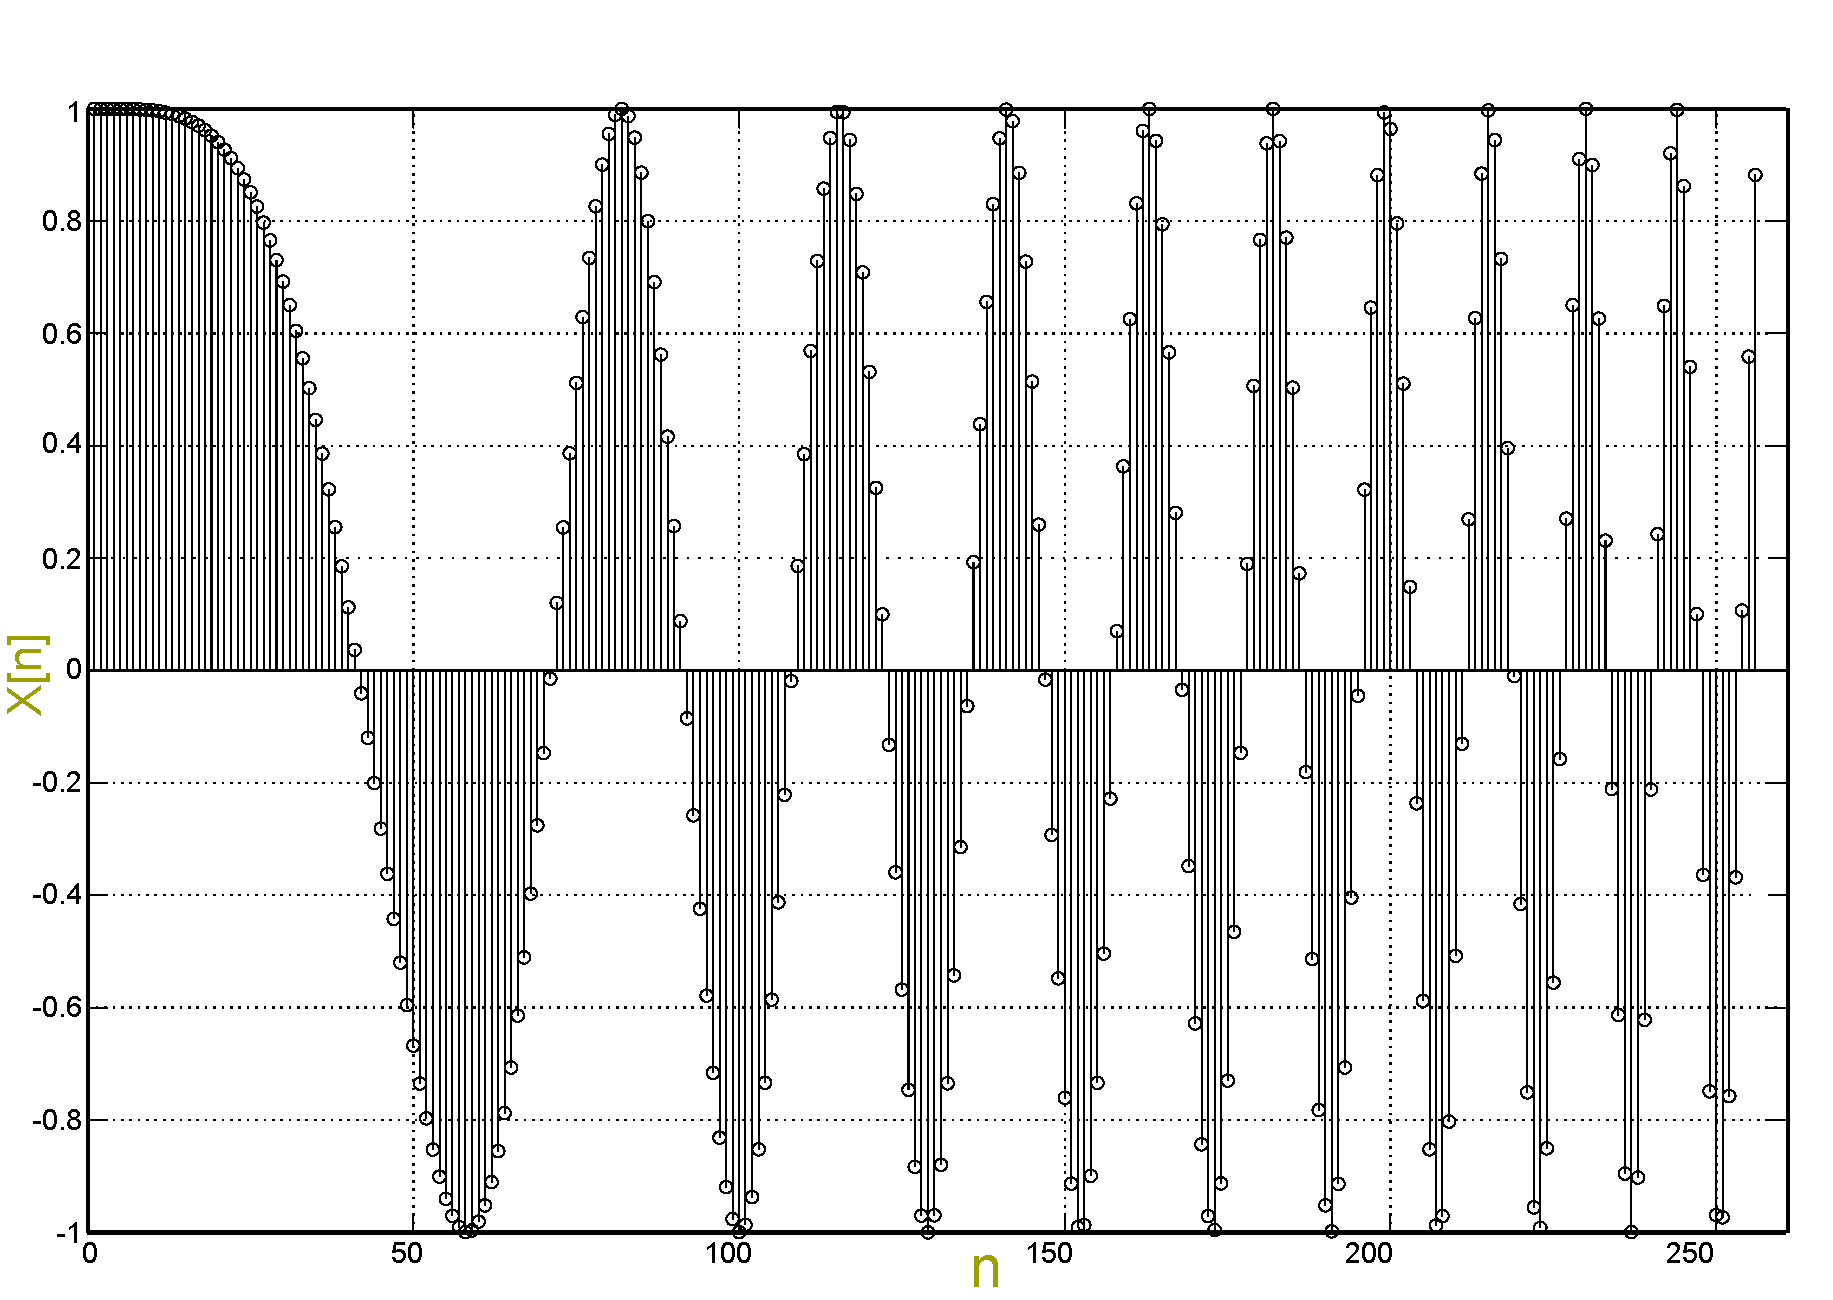
\includegraphics[width=0.8\linewidth]{Chirp_signal_stem.pdf} 
     \end{tabular}  
     \captionof{figure}{Chirp signál: Signál s lineárně rostoucím kmitočtem s maximální
              frekvencí 20 Hz vzorkovaný 254 Hz. Grafická reprezentace číslicových signálů bývá
              buď ve spojité formě (a) nebo v diskrétní formě (b) 
     \label{SAS:fig_chirp_sig}}
  \par}
  
  M-file:
  %---------------------------------------------------------------
  \lstinputlisting{../src/TKY/matlab/gen_chirp_signal.m}
  \begin{lstlisting}[caption=\texttt{gen\_chirp\_signal.m}. Generuje chirp signál]
  \end{lstlisting}
  %---------------------------------------------------------------
\end{example}